% ======================================================================
\section{Interpretation of the results}
\label{sec:interpretation}
% ======================================================================

This section explains what the features of the spectral functions and conductance maps of
\cref{sec:results} mean physically, and how the energy of the plasmon satellites can be estimated from
the plasmon dispersion. The numbers are produced by notebook 06 and \code{g0w.satellites}.

\subsection{What the spectral function contains}

$A(\bk,\eps)$ is the probability density for adding an electron of momentum $\bk$ at energy $\eps>0$ (or
removing one at $\eps<0$); $\int\dd\eps\,A=1$. In an interacting metal the added electron has two kinds of
final state:
\begin{itemize}
\item \textbf{the quasiparticle}: the electron dressed by a cloud of \emph{virtual} density fluctuations. It gives
the sharp peak at $E^*_{\bk}$ (\cref{sec:spectral}), with weight $Z<1$ ($Z\simeq0.82$--$0.83$ in doped graphene)
and displaced from the bare band by $\Ree\Sigma$;
\item \textbf{electron plus a real plasmon}: the electron enters by creating a plasmon $\bq$ and ends at
$\bk+\bq$. This costs $\eps=\xi_{\bk+\bq}+\omega_{\rm pl}(\bq)$, so the weight $1-Z$ is spread about one plasmon energy
away from the band. Where these final states pile up, $-\Imm\Sigma$ has a peak and $A$ a faint replica of the
band: the \emph{satellite}.
\end{itemize}
This is the electronic analogue of the phonon sidebands and shake-up satellites of photoemission, with the
plasmon in place of the phonon. Two consequences are general. The satellite of an empty state lies above the
quasiparticle peak and that of an occupied state below it: always on the side away from $E_F$. And the
satellite is not a separate particle and has no fixed energy of its own: it is the edge of a continuum, whose
position depends on the plasmon \emph{dispersion} and on the band, as quantified next. At the level of G$_0$W
only one satellite appears; replicas at multiples of the plasmon energy require higher-order (vertex or
cumulant) corrections.

\subsection{One-plasmon picture of $-\Imm\Sigma$}

Inserting the plasmon part of the spectral density, $S(\bq,\omega)\simeq R(\bq)\,\delta(\omega-\omega_{\rm pl}(\bq))$, into
the anti-Hermitian part of $\Sigma$ (\cref{sec:passivity}) gives for an empty state ($\eps>0$, $T=0$)
\begin{equation}
-\Imm\Sigma_{n}(\bk,\eps)\simeq\pi\sum_{\bq}w_{\bq}\sum_m\Theta(\xi_{m,\bk+\bq})\,
\bigl|\rho_{nm}(\bk,\bq)\bigr|^2_{R}\;\delta\bigl(\eps-E_{m\bk}(\bq)\bigr),\qquad
E_{m\bk}(\bq)=\xi_{m,\bk+\bq}+\omega_{\rm pl}(\bq),
\label{eq:onePlasmon}
\end{equation}
where $|\rho|^2_R=\sum_{ab}\rho^a_{nm}R_{ab}\rho^{b*}_{nm}$ (for graphene, the chirality factor times the residue). This
is a density of final states on the $\bq$ plane, weighted by the coupling. Like a density of states, it peaks
where the final energy $E_{m\bk}(\bq)$ is \emph{stationary} in $\bq$. The satellite energy is therefore a stationary
value of $E_{m\bk}(\bq)$, not $\omega_{\rm pl}$ at a particular $\bq$. \Cref{eq:onePlasmon} is used here only for
interpretation: all spectra of \cref{sec:results} are computed with the full spectral density of $W$, which also
contains the particle--hole continuum.

\subsection{Dispersive plasmon: the emission edge in graphene}
\label{sec:edge}

\paragraph{Estimate.} At fixed $q=|\bq|$, the direction of $\bq$ sweeps the final band energy
$\xi_{\bk+\bq}$ over $[\xi_{\bk}-\hbar v_Fq,\ \xi_{\bk}+\hbar v_Fq]$; the lowest value belongs to emission against the
electron's motion (the electron loses momentum along its velocity), and the angular density diverges at both
ends of the interval. The lower ends
\begin{equation}
E_-(q)=\xi_{\bk}+\omega_{\rm pl}(q)-\hbar v_Fq
\end{equation}
form a curve that, for a gapless 2D plasmon, first rises and then falls. At its maximum a whole range of $q$
starts contributing at the same energy (a caustic), the inverse-square-root singularities add up, and
$-\Imm\Sigma$ rises steeply. This is the emission edge:
\begin{equation}
\boxed{\eps_{\rm sat}\simeq\xi_{\bk}+\Delta,\qquad \Delta=\max_q\bigl[\omega_{\rm pl}(q)-\hbar v_Fq\bigr],\qquad
\left.\frac{d\omega_{\rm pl}}{dq}\right|_{q^*}=v_F}
\label{eq:edge}
\end{equation}
(\code{satellites.dispersive\_edge}). The maximum is reached where the plasmon group velocity equals the electron
velocity, a Cherenkov-like matching condition. The final state must be empty, $\xi_{\bk}-\hbar v_Fq^*\ge0$, i.e.
$|\bk|\ge k_F+q^*$; for smaller $|\bk|$ the edge is cut by Pauli blocking. For occupied states the mirror construction
gives $\eps_{\rm sat}\simeq\xi_{\bk}-\Delta$ for $|\bk|\le k_F-q^*$. Below the edge only small $q$ (small weight $w_qR$)
and large $q$ (Landau-damped plasmon) contribute, which is why $-\Imm\Sigma$ is small there.

\paragraph{Closed form.} For the long-wavelength plasmon $(\hbar\omega_{\rm pl})^2=\frac g2\frac{e^2}{\bar\varepsilon}E_Fq\equiv a^2q$,
maximising $a\sqrt q-\hbar v_Fq$ gives
\begin{equation}
q^*=\frac{a^2}{4(\hbar v_F)^2}=\frac g8\,\alpha_g\,k_F,\qquad
\Delta=\frac{a^2}{4\hbar v_F}=\frac g8\,\alpha_g\,E_F\ \stackrel{g=4}{=}\ \frac{\alpha_gE_F}{2},\qquad
\alpha_g=\frac{e^2}{\bar\varepsilon\hbar v_F}
\label{eq:edgeclosed}
\end{equation}
(\code{satellites.sqrt\_plasmon\_edge}): the satellite offset is a fraction of $E_F$ set by the graphene
fine-structure constant. For our junction ($\alpha_g=0.50$, $E_F=116.6$ meV) this gives $\Delta=29$ meV and
$q^*=0.25k_F$. The RPA plasmon of the junction lies above the $\sqrt q$ law at $q\sim0.4k_F$, and the full
dispersion gives larger values (\cref{tab:edge}).

\begin{figure}[htbp]
\centering
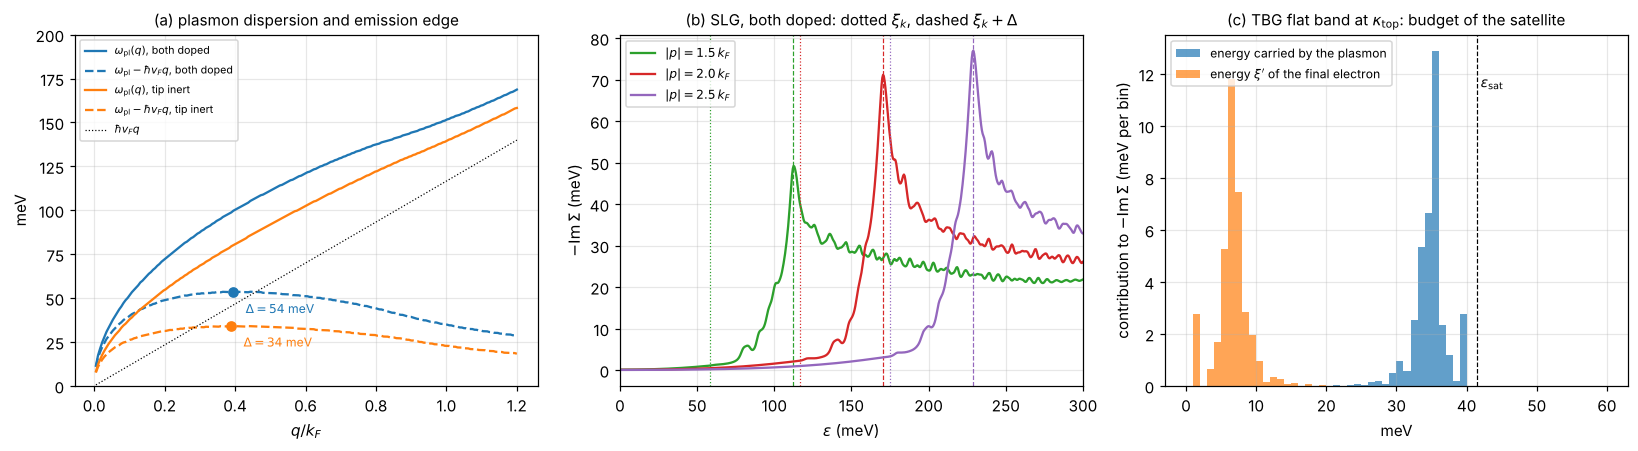
\includegraphics[width=\textwidth]{figures/fig_satellites.png}
\caption{(a) RPA plasmon dispersion of the sample sheet (solid) and $\omega_{\rm pl}(q)-\hbar v_Fq$ (dashed) for the doped and
the inert tip; dots: the maximum $\Delta$ of \cref{eq:edge}. (b) Full-frequency $-\Imm\Sigma$ of the conduction band at
three momenta (both sheets doped): the edge sits at $\xi_{\bk}+\Delta$ (dashed), one constant offset above the
bare band (dotted). (c) TBG, flat conduction band at $\kappa_{\rm top}$: decomposition of $-\Imm\Sigma$ at its peak
$\eps_{\rm sat}=41.5$ meV into the energy carried by the plasmon and the energy of the final electron.}
\label{fig:satellites}
\end{figure}

\begin{table}[htbp]
\centering
\small
\caption{Emission edge of the graphene sample: \cref{eq:edge} against the full-frequency calculation. All
energies in meV; $E^*$ is the quasiparticle peak of $A$.}
\label{tab:edge}
\begin{tabular}{lcccccccc}
\toprule
tip & $\Delta$ & $q^*/k_F$ & $|\bk|/k_F$ & $\xi_{\bk}$ & $\xi_{\bk}+\Delta$ & peak of $-\Imm\Sigma$ & satellite of $A$ & sat.\,$-\,E^*$\\
\midrule
doped & 53.7 & 0.40 & 1.5 & 58.3 & 112.0 & 112.5 & 115.0 & 73.0\\
      &      &      & 2.0 & 116.6 & 170.3 & 170.5 & 174.5 & 79.0\\
      &      &      & 2.5 & 174.9 & 228.6 & 229.0 & 233.0 & 82.0\\
inert & 34.1 & 0.39 & 1.5 & 58.3 & 92.4 & 92.5 & 95.5 & 53.5\\
      &      &      & 2.0 & 116.6 & 150.7 & 151.0 & 157.5 & 62.5\\
      &      &      & 2.5 & 174.9 & 209.0 & 209.0 & 215.0 & 64.5\\
\bottomrule
\end{tabular}
\end{table}

\paragraph{Check.} \Cref{eq:edge} reproduces the peak of the full-frequency $-\Imm\Sigma$ to within 0.5 meV at every
momentum (\cref{tab:edge,fig:satellites}b), and the plasmon slope at $q^*$ equals $v_F$ to 2\%. The satellite peak of $A$ lies
2--7 meV higher, pushed by the Dyson denominator $(\eps-\xi_{\bk}-\Ree\Sigma)^2$ of \cref{eq:Ascalar}.

\paragraph{Energy budget.} Neither $\omega_{\rm pl}(q^*)$ ($\simeq100$ meV) nor $\Delta$ ($\simeq54$ meV) is the energy of the emitted
plasmon. Decomposing $-\Imm\Sigma$ at the edge into the energy $\omega=\eps-\xi'$ carried away by the plasmon and the
energy $\xi'$ of the final electron (\code{satellites.slg\_energy\_loss}, $\eta\to0$): at $|\bk|=1.5k_F$ the plasmon
carries on average 82 meV (inter-quartile range 67--100 meV) and the electron ends at $\xi'\simeq30$ meV, with
momentum transfers around $0.3k_F$; at $2k_F$ the numbers are 96 meV (77--115 meV) and $\xi'\simeq75$ meV. The energy
of the added electron is shared between the plasmon and the drop of the electron's own band energy.

\paragraph{Offset seen in a QTM line cut.} A line cut measures the satellite relative to the quasiparticle peak,
\begin{equation}
\eps_{\rm sat}-E^*_{\bk}\simeq\Delta+\bigl(\xi_{\bk}-E^*_{\bk}\bigr)+\delta_D ,
\label{eq:offset}
\end{equation}
where $\xi_{\bk}-E^*_{\bk}=-\Ree\Sigma$ at the quasiparticle (16, 21 and 24 meV at $|\bk|=1.5$, 2 and $2.5k_F$) and
$\delta_D\simeq2$--$7$ meV is the Dyson shift. This accounts for the offsets of \cref{fig:qtmslgcuts}:
\begin{itemize}
\item \textbf{Plateau.} $\Delta$ does not depend on $\bk$, so the offset grows only through the slowly increasing
$-\Ree\Sigma$ and is nearly constant at large $\theta$: $\simeq80$ meV with a doped tip, $\simeq63$ meV with an inert one.
\item \textbf{Onset.} The edge needs $|\bk|\ge k_F+q^*\simeq1.4k_F$, i.e.\ $\theta\gtrsim1.4\,\theta(k_F)=0.83^\circ$
(\cref{eq:ptheta}); below that the edge is Pauli-blocked and the offset is smaller, as in the rising part of the
curve.
\item \textbf{Tip back-action.} Doping the tip raises $\Delta$ from 34.1 to 53.7 meV; together with the slightly
larger Dyson shift of the inert case this gives the 17 meV increase of the QTM offset. The tip's carriers oscillate in phase with the sample's in the optical
plasmon of the junction, adding Drude weight and stiffening its dispersion (in the limit $qd\to0$ the in-phase
mode of two identical sheets has twice the Drude weight, $a^2\to2a^2$, which would double $\Delta$; at $q^*$ the
computed ratio is 1.57). The satellite energy therefore depends on the electrostatic environment of the
sample, including the probe.
\end{itemize}
Because $\Sigma$ contains only the correlation part (\cref{sec:exchange}), the quasiparticle shift in
\cref{eq:offset} is correlation-only; the Fock term would move $E^*$ but not $\eps_{\rm sat}$.

\subsection{Flat plasmon and flat bands: twisted bilayer graphene}
\label{sec:flatsat}

In TBG at $1.2^\circ$ both the plasmon and the final states are nearly dispersionless: the peak of the sample
spectral density is at $34.2$ meV over the whole moir\'e mesh (inter-quartile range 32.7--35.2 meV), and the flat bands
are $\simeq25$ meV wide. The $\bq$ integral then hardly matters, and the stationary value of $E_{m\bk}(\bq)$ is reached
where the density of final flat-band states peaks, at the van Hove energy $\xi_{\rm VH}$:
\begin{equation}
\boxed{\eps_{\rm sat}\simeq\pm\bigl(\xi_{\rm VH}+\bar\omega_{\rm pl}\bigr)}
\label{eq:flatsat}
\end{equation}
With $\xi_{\rm VH}=6.2$ meV (peak of the conduction flat-band DOS) this gives 40.5 meV, against the computed peak of
$-\Imm\Sigma$ of the flat band at $\kappa_{\rm top}$, 41.5 meV. The decomposition (\code{satellites.tbg\_energy\_loss},
\cref{fig:satellites}c) confirms the picture: the plasmon carries $34.8$ meV on average (inter-quartile range
33.8--35.6 meV) and all final states lie in the flat band, at $\xi'\simeq6.7$ meV. The satellite of $A$ and of
$dI/dV$ appears at $|eV|\simeq45$ meV, again a few meV beyond the peak of $-\Imm\Sigma$ because of the Dyson
denominator. The hole satellite is the mirror image, by the approximate particle--hole symmetry of the
continuum bands.

Since neither $\bar\omega_{\rm pl}$ nor $\xi_{\rm VH}$ depends on $\bk$, the satellite energy is the same at every momentum
probed by the tip. This is why, in \cref{fig:qtmtbgmap,fig:qtmtbgcuts}, the satellites form horizontal stripes
that do not move with the twist angle, while the quasiparticle peaks follow the bands along the trajectory
(zero bias at $\kappa_{\rm top}$ and $\kappa_{\rm bot}$, $\pm12$ meV at $\gamma'$). The angle independence is the
fingerprint that distinguishes a flat-plasmon satellite from a band.

\subsection{What a QTM measurement of the satellites determines}

Since $dI/dV\propto\bra{\chi_\theta}A(\bK_\theta,eV)\ket{\chi_\theta}$ (\cref{eq:didv}), the quasiparticle ridges of a map give the
renormalised bands and the satellites give the one-plasmon emission edges. In graphene the satellite
offset is not the plasmon energy but $\Delta=\max_q[\omega_{\rm pl}-\hbar v_Fq]$, a property of the plasmon dispersion
near the momentum where its slope equals $v_F$, plus the quasiparticle shift of \cref{eq:offset}; extracting
plasmon information from it requires either the measured quasiparticle ridge and band velocity, or the
calculation. In flat-band TBG the offset is close to $\bar\omega_{\rm pl}+\xi_{\rm VH}-E^*_{\bk}$, a nearly direct, angle-independent
measure of the flat-band plasmon energy. In both cases the edge is sharpened in $d^2I/dV^2$, and its position
depends on the screening environment, the tip included.
